\chapter{系统架构}

\section{系统总览}

本文提出了一种基于“慢思考”与“快反应”双层架构的交通智能体系统。整个系统由慢思考层和快反应层组成，两者之间通过信息流协同工作，共同完成从用户指令到交通分析结果的完整处理流程。

\begin{figure}[H]
  \centering
  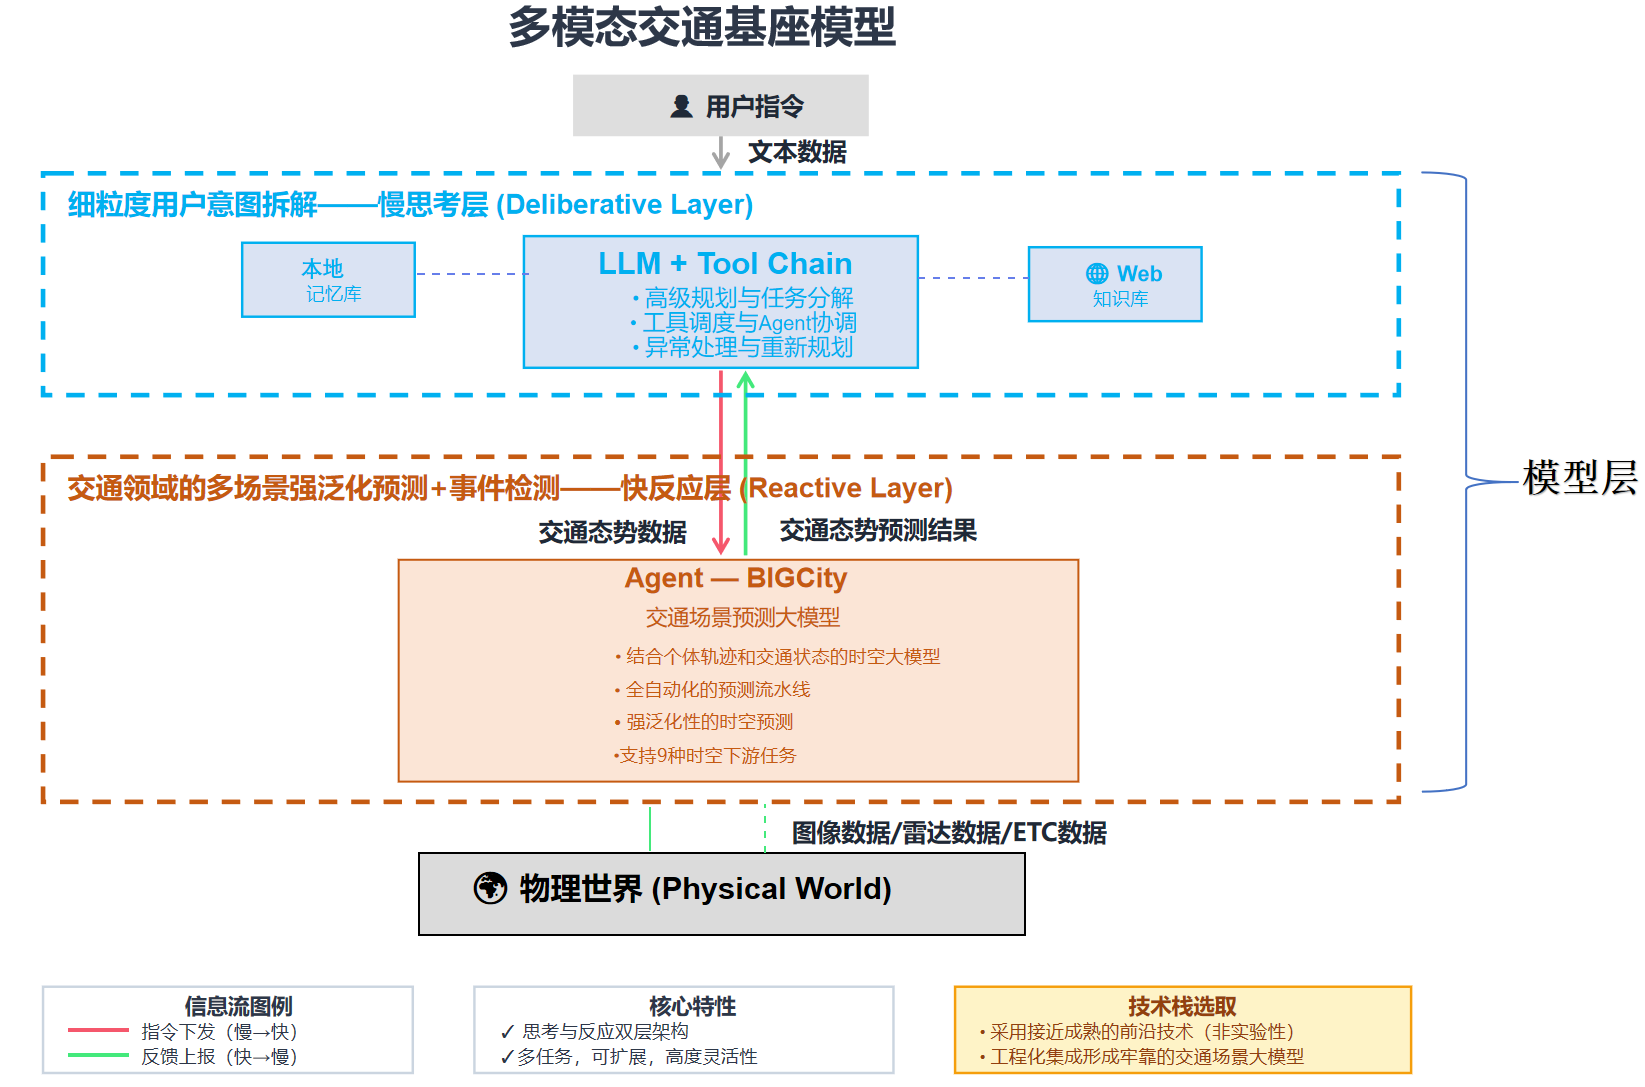
\includegraphics[width=0.9\textwidth]{figure/image15.png}
  \caption{系统总体架构图}
  \label{fig:system-architecture}
\end{figure}

系统的上层为慢思考层。这一层用大语言模型做复杂的多步推理和规划的任务。当用户通过自然语言输入交通管理相关指令的时候，慢思考层会先对指令进行语义解析以及细粒度的意图拆解。它把用户的模糊描述变成一个个可以执行的子任务，再把子任务的执行步骤按逻辑顺序排列起来。慢思考层会存贮起历史交互记录以及上下文信息，从而保证智能体在多次对话或者繁杂任务当中可以维持对于任务状况的正确认识。大语言模型依靠系统提示词以及记忆库里的信息来执行高级规划与任务拆解，工具调度以及Agent协调，异常应对并动态重新规划等工作。若在执行中出现工具调用失败或者返回数据不符合预期等情况，慢思考层会依照目前的执行状况去重新安排后面的计划，不会因为这些异常而终止整个流程。

系统的下层是快反应层，属于整个系统的模型层。这一层聚焦于交通领域的数值计算和快速预测任务，由Agent调度模块和BIGCity时空预测模型共同组成。BIGCity是一个结合了路网个体轨迹数据和交通状态数据的时空预测大模型，专门用于从多源交通数据中提取时空特征并输出准确的预测结果 \upcite{ref62_yu2025bigcity}。在具体使用上，本系统主要用到了BIGCity的交通流量预测功能——预测未来一段时间内路网中各路段的车流量变化趋势，为智能体的分析和决策提供定量依据。

BIGCity有三个主要的特性。第一个就是全自动的预测流水线。系统从多源原始数据加载开始，就可以自动完成缺失值填充、时间对齐、标准化处理、原子文件格式化、时空特征矩阵构建等任务，最后输出预测结果。整个过程不需要人工干预，用户只需发出查询请求，系统就会自动完成从数据到预测的全部过程。第二个就是强泛化性。交通数据在不同城市的分布是不一样的，在不同路网结构的城市间迁移的时候，传统模型的性能会急剧下降。BIGCity模型的设计将路网个体轨迹数据和交通状态数据这两种不同的尺度信息融合起来，使得模型可以学习到更加通用的时空依赖模式，而不会因为局部结构的过度拟合而产生偏差。这说明模型对于新的路网、新的交通模式有更强的适应性。第三个是结合个体轨迹与交通状态的建模能力。BIGCity的输入不是路段级的流量统计，还有个体车辆的GPS轨迹信息。轨迹数据可以提供细粒度的车辆行为信息，即每辆车的行驶路径、速度、停留时间等，交通状态数据可以给出路段级别的聚合统计，如流量、速度、占有率等。两者结合使得模型可以同时看到每辆车的微观行为以及整个路网的宏观状况，进而作出更加准确的预测。

慢思考层和快反应层之间依靠双向信息流进行协作。指令下发方向是从慢到快，慢思考层把用户的意图分解成具体的计算或者查询请求，然后发送给快反应层去执行。反馈上报方向为从快到慢，快反应层把计算结果和预测数据传回慢思考层，再由慢思考层对大模型进行分析、综合，最后生成最终的文本报告。分层协作的设计使系统在面对需要多步推理的复杂问题的时候可以调动大模型的语义理解能力，在处理常规的数值查询、预测请求的时候可以绕过耗时的推理过程，直接使用快反应层来快速响应，既保证了系统的智能性又提高了系统的响应速度。

系统整体用模块化设计思想，各个功能模块可以独立替换和升级。慢思考层的核心大模型可以按照需要选择不同的模型，快反应层的预测模型也可以接入不同的交通预测算法。解耦方式可以使得系统对于新的交通场景以及业务需求有较好的扩展性。


\section{慢思考层}

慢思考层是系统的核心推理和规划模块，它的工作机制可以理解为大语言模型加工具调用（LLM+Tool Calling）。大模型不会直接用自己训练的知识去回答交通问题，它会调用外部的工具去获取实时的数据和计算的结果，再根据这些信息进行分析和决策。该种设计有两个优点，第一，可以避免由于训练数据时间截止而给出过时信息的情况，例如用户询问当前的拥堵情况，训练数据中包含的数据可能是几个月前的，直接回答毫无意义；第二，每一步分析都有真实的数据显示作依据，不是模型凭空产生的数字，用户可以看到数据来源，结果更可信。系统提示词中规定了所有的可用工具的接口格式以及调用规范，大模型按照这些规范调度工具，不会超过系统所规定的限制。

当用户的自然语言指令进入到慢思考层之后，系统就会对指令展开语义解析以及意图识别。系统提示词中给出了可以使用的工具接口及调用规范，大模型根据提示词从用户描述中提取出需要查询的路段编号、时间范围、分析目的等参数。自然语言中时间表达方式多样，有“今天早高峰”“下午三点”“2024年6月15号上午”等，都需要模型统一解析成系统内部使用的格式。模型把宏观任务拆解成具体的子任务序列，用户说“对比一下北三环和西二环今天早高峰的拥堵情况”，模型就会解析出两个路段ID、时间范围为早高峰时段、分析目的为拥堵对比，然后拆解成三步，第一步查询两个路段的实时流量数据，第二步获取对应的历史趋势，第三步对比分析并生成报告。

任务分解之后，系统就会进入到工具调用的执行阶段。大模型在一个推理过程中可以发出许多工具调用指令，这些指令会被同时发送到底层的工具执行节点上。LangGraph的ToolNode节点收到多个工具调用请求之后，就会同时执行所有的不冲突调用，而不是一个一个地串行等待。拥堵对比任务中模型可以对北三环和西二环进行实时查询，两个查询互相独立，可以并行处理。并行机制可以减小响应时间，串行执行两个查询要分别进行一次网络往返和模型两次推理，总耗时最少也要翻一番。工具执行节点把所有的调用结果一起返回给模型，模型再根据返回的信息继续进行下一轮的推理。

慢思考层的循环执行逻辑基于LangGraph框架的状态图（StateGraph）来实现。系统定义了两个核心的图节点。第一个是大模型推理节点（agent），负责根据当前的任务状态和已经获取的信息生成下一轮的工具调用指令或者直接输出最终的分析报告。第二个是工具执行节点（execute\_tools），负责接收并执行模型发出的工具调用指令。两个节点之间通过条件路由边连接：每次agent节点执行完毕后，系统检查模型输出中是否包含有效的工具调用指令。如果包含，就路由到execute\_tools节点执行工具，执行完成后再回到agent节点继续推理。如果模型判断信息已经足够、直接输出了分析报告，循环就结束。这个“推理→执行→观察→再推理”的循环确保了系统能够在复杂的、需要多步操作的任务中逐步推进。每一步都能看到上一步的结果，根据实际情况动态调整后续步骤，而不是按照预先写死的流程走到底。

当使用工具调用的目标数据源不可用，或者查询参数格式有误的时候会出现错误信息。当出现异常的时候，大模型推理节点会得到工具执行节点返回的错误信息，模型根据错误类型来改变后面策略。如果参数有误，模型就会重新考虑，修正参数之后再发起调用。如果数据源不可用，模型就会选择跳过这个步骤或者使用备份的数据来源。用户询问西直门桥的实时流量，但是西直门桥下辖有多个方向的路段，第一次调用由于参数范围不明而失败。模型收到错误之后就会把查询拆分成分方向的子请求，然后分别调用后合并结果。如果某个方向的数据源正好离线，模型就会忽略该方向的数据，用其他方向的数据来给出部分分析结果，而不是直接报错。该种异常处理机制可以保证系统在真实的环境下具有鲁棒性，不会因为单个工具的临时故障而使整个任务中断。

另外慢思考层还有一个记忆库来保存目前的对话历史交互记录以及中间计算结果。该记忆库利用LangGraph框架的状态累积特性来完成，每一轮对话中用户发出的消息、模型给出的回答以及工具给出的结果都会被自动加入到状态里，之后的轮次可以直接调用。记忆库可以保证对话多次进行的时候，模型不会丢失上下文。用户先提出某路段的路况问题，然后又提出了“旁边”的问题，模型可以从中知道前面一个问题是指哪个路段，进而对“旁边”所指代的关系做出正确的理解。除了消解指代之外，记忆库还有着另外一个重要的作用，那就是当用户在一段对话中多次查询同一路段在不同时间段的流量时，模型就不需要每次都重新解析完整的路段信息了，而是可以从记忆中读取之前已经确认过的路段参数，直接组装新的查询请求。这减小了重复的参数解析环节，也缩减了在多轮对话里模型理解出现失误的可能性。

\section{快反应层}

快反应层是系统的数值计算引擎，负责处理交通流量的快速预测和实时数据查询。它的核心是一个名为BIGCity的时空交通流量预测大模型，专门用于从多源交通数据中提取时空特征并输出准确的预测结果。

BIGCity是把路网个体轨迹数据和交通状态数据结合起来形成的时空大模型。与传统的交通预测模型相比，它不是只对某一条道路的流量进行预测，而是一套全自动化的预测流水线。原始多源交通数据来源于物理世界各种采集设备，道路传感器采集的车流量、速度、占有率数据，雷达设备采集的车辆通行数据，ETC系统采集的收费数据。数据进入快反应层之后首先要经过数据清洗、标准化处理变为原子文件，对缺失值和异常值进行插补和修正，再根据路网拓扑结构把分散的传感器数据映射到全局图结构上，组装成统一的时空特征矩阵，最后输入模型进行推理。整个从原始数据到预测结果输出的过程都是自动化完成的，不需要人工干预。

BIGCity的一个主要特点就是支持各种各样的时空下游任务。传统的交通预测模型大多只针对单一的预测任务进行设计，即专门预测车流量或者专门预测通行速度，一旦更换了任务，就需要重新训练模型。BIGCity用统一的时空表示学习框架可以同时对轨迹预测、流量预测、速度预测、出行需求预测等九种不同的时空任务进行处理。这就意味着系统对于各种各样的交通分析需求，都不需要为每一个需求单独搭建起一个预测模型，而是一个模型就能涵盖所有的情况。本系统主要研究的是时空预测的功能。另外BIGCity还有全自动化的预测流水线，从数据加载、特征提取、模型推理到最后的结果输出都是系统自动完成的，用户不需要去关注模型具体是怎么运作的。

另一个特点就是强泛化性。交通数据在各个城市、各个区域的分布情况不一样，一个在A城市训练好的模型搬到B城市的时候性能会明显降低。BIGCity模型设计考虑到了跨域泛化的因素，将个体轨迹数据和交通状态数据两种不同的尺度的信息结合起来使用，从而使得模型能够学到比较通用的时空依赖模式，而不是过分贴合某一个路网的局部特性。系统所使用的原子文件格式(.geo、.rel、.dyna)也给跨域泛化提供了一个数据支持。无论数据来自哪个城市或者传感器网络，原子文件都是用同样的格式来组织的，即.geo描述实体的位置、.rel描述连接关系、.dyna描述动态状态。不同的来源的数据在进入系统的时候已经完成了格式统一，模型所面对的数据结构一直是一致的，不需要为每一个城市单独编写数据加载和预处理的代码。这就意味着模型可以同时在各个城市的数据上进行联合训练，也可以在一个城市训练之后直接迁移到另一个城市使用，只要新城市的数据按照相同的原子文件格式组织起来即可。格式统一加上模型本身的跨域设计，使系统对于新的路网结构或者交通模式有更强的适应性。

技术上使用了基于自注意力机制的Transformer结构来建模交通数据的时空依赖性。与传统的图神经网络相比，它有着明显的优势。第一是动态空间建模能力。传统的邻接矩阵只用固定的方式表示路网中路段之间的连接关系，而实际上路段之间相互影响是随时间、交通状况的变化而变化的。高峰期的拥堵路段和平峰期的通畅路段对周围路网的影响是不同的。自注意力机制可以依据目前的交通状况动态计算各个路段之间的相关程度，使得模型能自适应地关注到最相关的空间依赖关系。

第二就是长距离依赖的捕捉能力。传统的图卷积方法一般只聚合相邻节点的信息，经过多层堆叠才能间接获得远距离的信息，在信息传播的过程中容易发生衰减。自注意力机制让每一个路段都能够对路网中其它所有路段的状态进行直接的观察，而不论这些路段是否处于拓扑意义上的同一个位置。这在交通预测中十分重要，因为城市路网上远距离的路段之间确实存在着流量相关性，即快速路一个入口发生拥堵会波及数公里外的路段的通行情况。

第三就是对传播延迟的建模。交通状况在路网中传播并不是瞬间完成的，拥堵从上游路段传到下游路段要经过一段时间，这段时间与路段长度、当前车速有关。BIGCity在建模的时候考虑到传播延迟特性，从而使得模型可以更好地推断出交通态势在路网上扩散的过程。综上所述，这些技术特点使BIGCity对于复杂的交通模式有更强的捕捉能力，在节假日、大型活动、突发事件等非常规交通场景下也能得到较好的预测结果。

从系统集成角度来说，快反应层是作为一个独立的计算模块存在的，它通过标准接口同上层的慢思考层进行通信。慢思考层下发预测请求的时候，快反应层会自动生成特征组装、模型推理以及结果返回的过程。预测请求到达之后，快反应层就会遍历目标路段以及其相邻路段，从数据库里获取过去一小时的流量序列，每一个数据点都是五分钟一次，一共有十二个时间步。最后把所有的路段数据按照时间戳进行对齐，得到完整的时空特征矩阵，输入BIGCity模型进行推理，得到未来一个小时全路网流量预测结果。最后根据结果得到目标路段对应的预测序列，用结构化的JSON格式返回给慢思考层。